\style{ft}

\section{Mémo Mu-Editor pour \mbpy}



\begin{methode}[Mon 1er programme]
	\begin{multicols}{2}
		Affichons un premier texte sur l'écran du \mb.
	
		\textbf{Connecter} la carte à l'ordinateur
		\\[1em]
		
		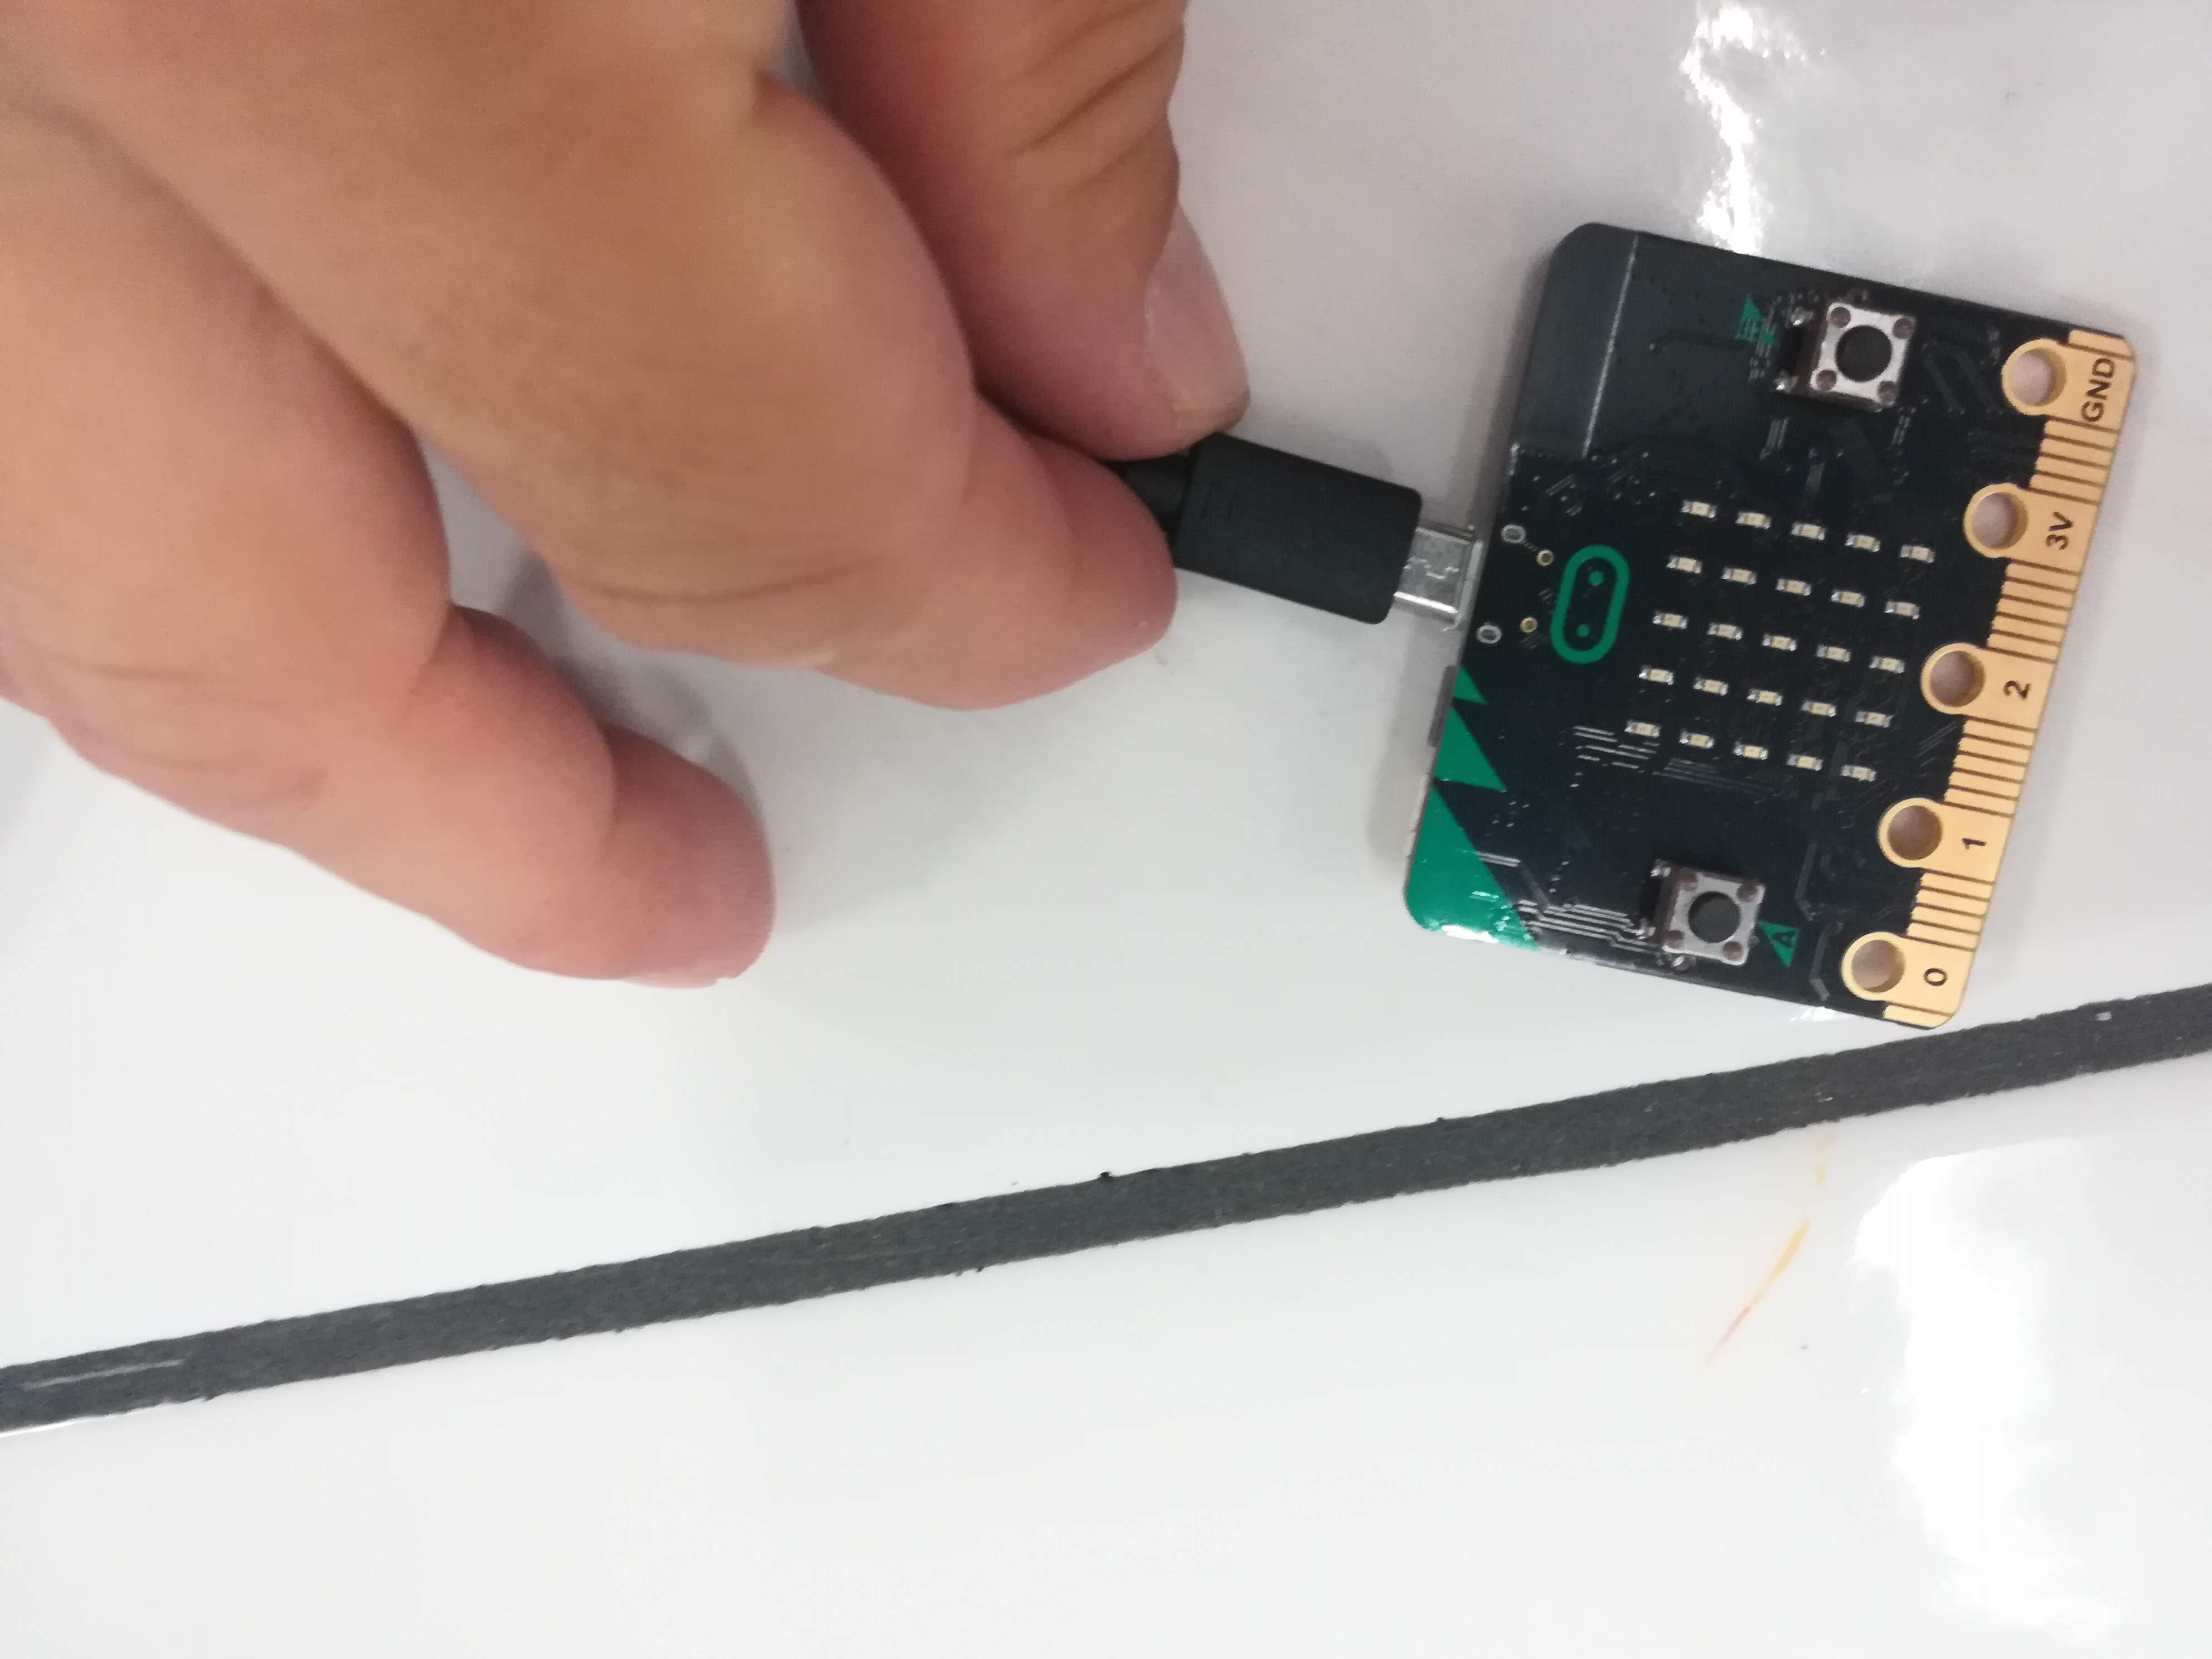
\includegraphics[height=10em]{res/mu/005.jpg}
		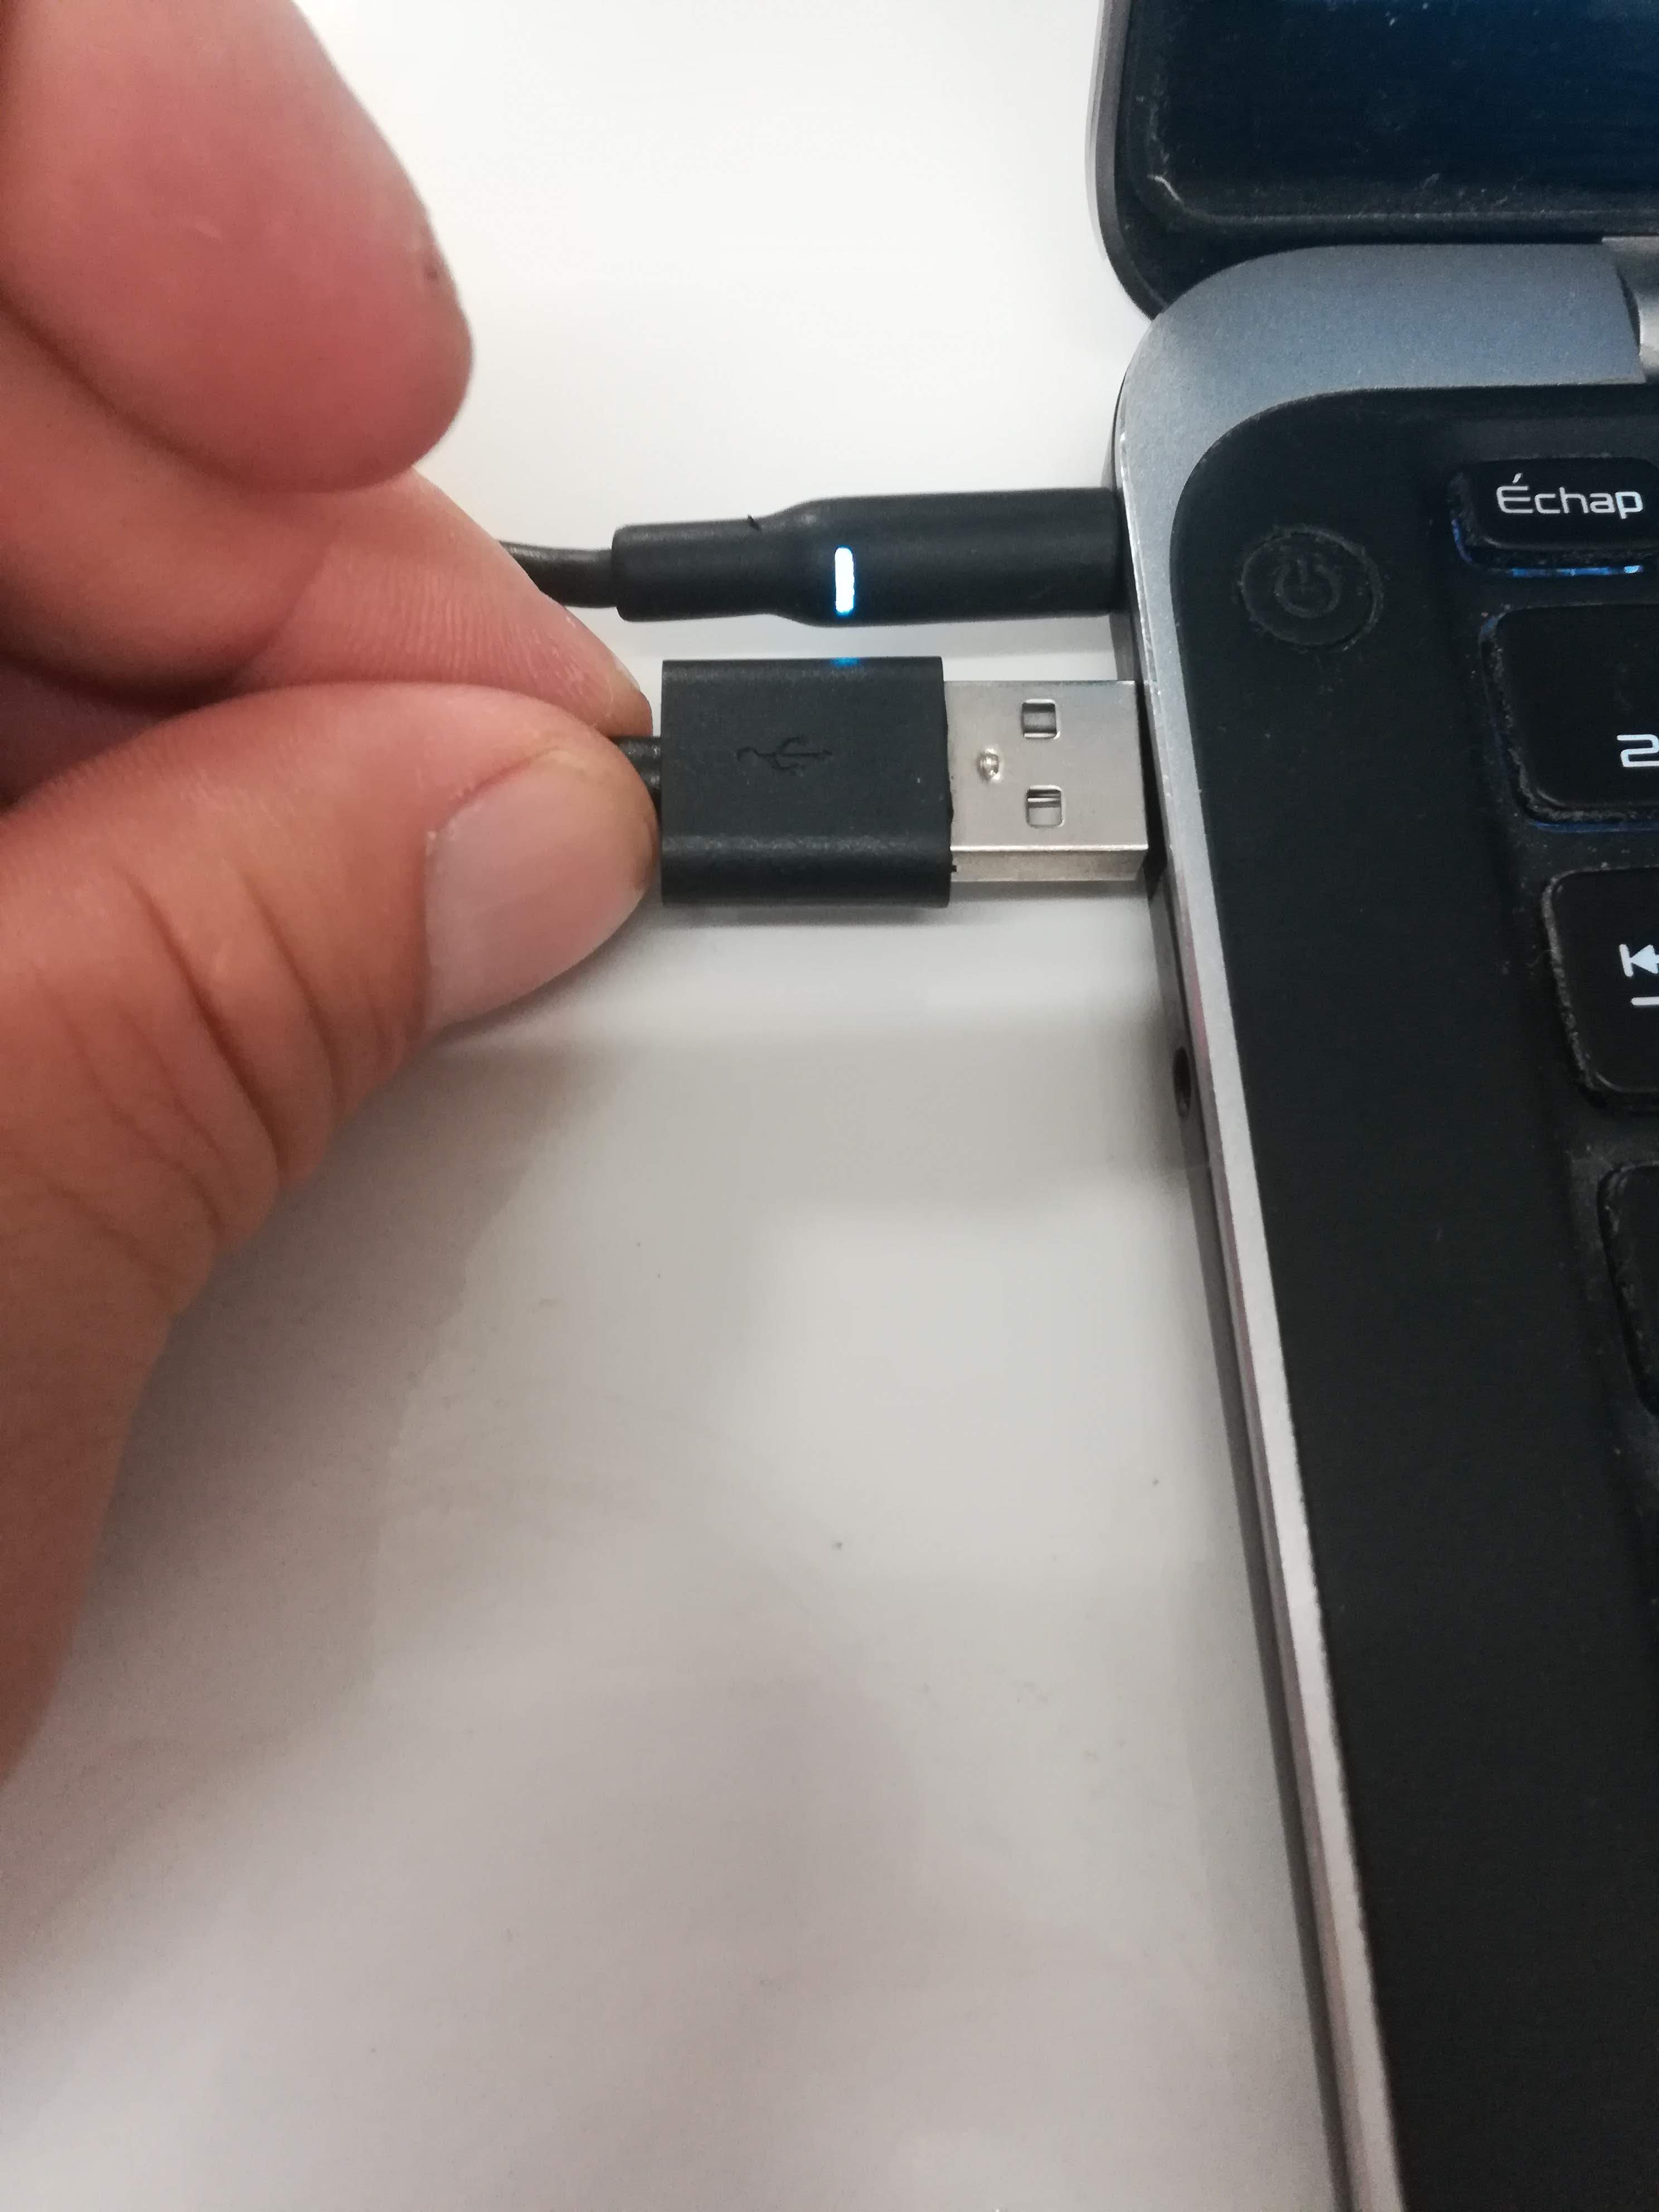
\includegraphics[height=10em]{res/mu/006.jpg}
		
	\columnbreak


	\textbf{Ouvrir} Mu-editor\\
	\textbf{Copier} le code ci-dessous.

	\begin{mucode}
from microbit import *
display.scroll("Hello, World!")
	\end{mucode}

	\textbf{Flasher} la carte (envoyer le programme dans 
	la carte)\\
	\hfill 
\includegraphics[width=5em]{res/flash.png}

	\end{multicols}
\end{methode}

	


\begin{methode}[Des images]

	\begin{multicols}{2}

		Affichons une image sur l'écran du \mb.

		\textbf{Copier} le code ci-dessous.

\begin{mucode}
from microbit import *
for loop in range (10):
	display.show(Image.HEART)
	sleep(100)
	display.show(Image.HEART_SMALL)
	sleep(50)
display.scroll("Hello, World!")
\end{mucode}

		\columnbreak
		
		\begin{center}
		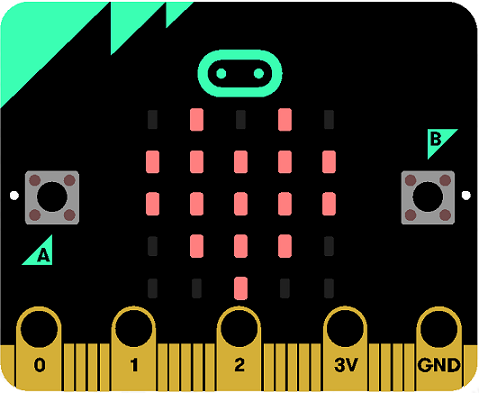
\includegraphics[width=9em]{res/mbpy-init-heart.png}
		\end{center}

		\textbf{Flasher} la carte
		\hfill
\includegraphics[width=5em,valign=c]{res/flash.png}
		
	\end{multicols}
\end{methode}



qsdf qsdf sdqf sdqf sq f sqdf sqdf sdqf sdqf sdqf sqdf  sqd fqsdf sqd fsqd fsqd fsqdf sdq sqdf
qsdf qsdf sdqf sdqf sq f sqdf sqdf sdqf sdqf sdqf sqdf  sqd fqsdf sqd fsqd fsqd fsqdf sdq sqdf
qsdf qsdf sdqf sdqf sq f sqdf sqdf sdqf sdqf sdqf sqdf  sqd fqsdf sqd fsqd fsqd fsqdf sdq sqdf
qsdf qsdf sdqf sdqf sq f sqdf sqdf sdqf sdqf sdqf sqdf  sqd fqsdf sqd fsqd fsqd fsqdf sdq sqdf
qsdf qsdf sdqf sdqf sq f sqdf sqdf sdqf sdqf sdqf sqdf  sqd fqsdf sqd fsqd fsqd fsqdf sdq sqdf
qsdf qsdf sdqf sdqf sq f sqdf sqdf sdqf sdqf sdqf sqdf  sqd fqsdf sqd fsqd fsqd fsqdf sdq sqdf
qsdf qsdf sdqf sdqf sq f sqdf sqdf sdqf sdqf sdqf sqdf  sqd fqsdf sqd fsqd fsqd fsqdf sdq sqdf
qsdf qsdf sdqf sdqf sq f sqdf sqdf sdqf sdqf sdqf sqdf  sqd fqsdf sqd fsqd fsqd fsqdf sdq sqdf
qsdf qsdf sdqf sdqf sq f sqdf sqdf sdqf sdqf sdqf sqdf  sqd fqsdf sqd fsqd fsqd fsqdf sdq sqdf
qsdf qsdf sdqf sdqf sq f sqdf sqdf sdqf sdqf sdqf sqdf  sqd fqsdf sqd fsqd fsqd fsqdf sdq sqdf
qsdf qsdf sdqf sdqf sq f sqdf sqdf sdqf sdqf sdqf sqdf  sqd fqsdf sqd fsqd fsqd fsqdf sdq sqdf
qsdf qsdf sdqf sdqf sq f sqdf sqdf sdqf sdqf sdqf sqdf  sqd fqsdf sqd fsqd fsqd fsqdf sdq sqdf

qsdf qsdf sdqf sdqf sq f sqdf sqdf sdqf sdqf sdqf sqdf  sqd fqsdf sqd fsqd fsqd fsqdf sdq sqdf
qsdf qsdf sdqf sdqf sq f sqdf sqdf sdqf sdqf sdqf sqdf  sqd fqsdf sqd fsqd fsqd fsqdf sdq sqdf
qsdf qsdf sdqf sdqf sq f sqdf sqdf sdqf sdqf sdqf sqdf  sqd fqsdf sqd fsqd fsqd fsqdf sdq sqdf
qsdf qsdf sdqf sdqf sq f sqdf sqdf sdqf sdqf sdqf sqdf  sqd fqsdf sqd fsqd fsqd fsqdf sdq sqdf
qsdf qsdf sdqf sdqf sq f sqdf sqdf sdqf sdqf sdqf sqdf  sqd fqsdf sqd fsqd fsqd fsqdf sdq sqdf
qsdf qsdf sdqf sdqf sq f sqdf sqdf sdqf sdqf sdqf sqdf  sqd fqsdf sqd fsqd fsqd fsqdf sdq sqdf
qsdf qsdf sdqf sdqf sq f sqdf sqdf sdqf sdqf sdqf sqdf  sqd fqsdf sqd fsqd fsqd fsqdf sdq sqdf
qsdf qsdf sdqf sdqf sq f sqdf sqdf sdqf sdqf sdqf sqdf  sqd fqsdf sqd fsqd fsqd fsqdf sdq sqdf
qsdf qsdf sdqf sdqf sq f sqdf sqdf sdqf sdqf sdqf sqdf  sqd fqsdf sqd fsqd fsqd fsqdf sdq sqdf
qsdf qsdf sdqf sdqf sq f sqdf sqdf sdqf sdqf sdqf sqdf  sqd fqsdf sqd fsqd fsqd fsqdf sdq sqdf
qsdf qsdf sdqf sdqf sq f sqdf sqdf sdqf sdqf sdqf sqdf  sqd fqsdf sqd fsqd fsqd fsqdf sdq sqdf
qsdf qsdf sdqf sdqf sq f sqdf sqdf sdqf sdqf sdqf sqdf  sqd fqsdf sqd fsqd fsqd fsqdf sdq sqdf


\begin{methode}[Les mouvements]
	Affichons maintenant les mesures enregistrées
	par \textbf{l'accéléromètre}
\begin{multicols}{2}

	\textbf{Copier} le code ci-dessous
	\begin{mucode}
from microbit import *
display.show(Image.YES)
while True:
    valeurs= accelerometer.get_values()
    print (valeurs)
    sleep(100)
	\end{mucode}

	\textbf{Flasher} la carte 
	\hfill
\includegraphics[width=3em,valign=t]{res/flash.png}

	Afficher la vue \textsc{repl} (\textbf{terminal série})
	\hfill
\includegraphics[width=3em,valign=t]{res/ft_repl.png}

	\textbf{Réinitialiser} le \mb
	\hfill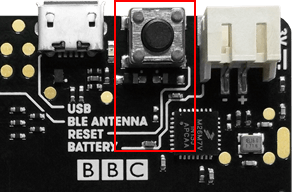
\includegraphics[width=7em,valign=c]{res/mu/060.png}

\end{multicols}
\end{methode}

qsdf qsdf sdqf sdqf sq f sqdf sqdf sdqf sdqf sdqf sqdf  sqd fqsdf sqd fsqd fsqd fsqdf sdq sqdf
qsdf qsdf sdqf sdqf sq f sqdf sqdf sdqf sdqf sdqf sqdf  sqd fqsdf sqd fsqd fsqd fsqdf sdq sqdf
qsdf qsdf sdqf sdqf sq f sqdf sqdf sdqf sdqf sdqf sqdf  sqd fqsdf sqd fsqd fsqd fsqdf sdq sqdf
qsdf qsdf sdqf sdqf sq f sqdf sqdf sdqf sdqf sdqf sqdf  sqd fqsdf sqd fsqd fsqd fsqdf sdq sqdf
qsdf qsdf sdqf sdqf sq f sqdf sqdf sdqf sdqf sdqf sqdf  sqd fqsdf sqd fsqd fsqd fsqdf sdq sqdf
qsdf qsdf sdqf sdqf sq f sqdf sqdf sdqf sdqf sdqf sqdf  sqd fqsdf sqd fsqd fsqd fsqdf sdq sqdf
qsdf qsdf sdqf sdqf sq f sqdf sqdf sdqf sdqf sdqf sqdf  sqd fqsdf sqd fsqd fsqd fsqdf sdq sqdf
qsdf qsdf sdqf sdqf sq f sqdf sqdf sdqf sdqf sdqf sqdf  sqd fqsdf sqd fsqd fsqd fsqdf sdq sqdf
qsdf qsdf sdqf sdqf sq f sqdf sqdf sdqf sdqf sdqf sqdf  sqd fqsdf sqd fsqd fsqd fsqdf sdq sqdf
qsdf qsdf sdqf sdqf sq f sqdf sqdf sdqf sdqf sdqf sqdf  sqd fqsdf sqd fsqd fsqd fsqdf sdq sqdf
qsdf qsdf sdqf sdqf sq f sqdf sqdf sdqf sdqf sdqf sqdf  sqd fqsdf sqd fsqd fsqd fsqdf sdq sqdf
qsdf qsdf sdqf sdqf sq f sqdf sqdf sdqf sdqf sdqf sqdf  sqd fqsdf sqd fsqd fsqd fsqdf sdq sqdf

\begin{remarque}
	Vous devriez avoir un affichage du type\\
		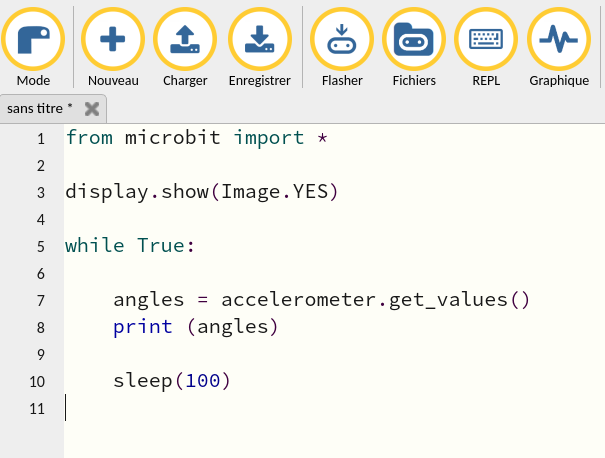
\includegraphics[width=0.5\linewidth,valign=t]{res/mu/050.png}
		\hfill
		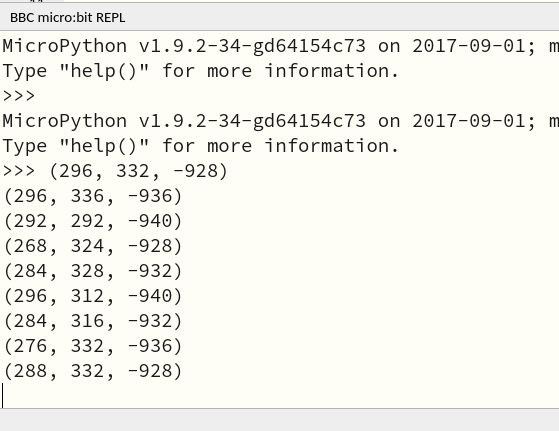
\includegraphics[width=0.5\linewidth,valign=t]{res/mu/070.png}	
\end{remarque}



qsdf qsdf sdqf sdqf sq f sqdf sqdf sdqf sdqf sdqf sqdf  sqd fqsdf sqd fsqd fsqd fsqdf sdq sqdf
qsdf qsdf sdqf sdqf sq f sqdf sqdf sdqf sdqf sdqf sqdf  sqd fqsdf sqd fsqd fsqd fsqdf sdq sqdf
qsdf qsdf sdqf sdqf sq f sqdf sqdf sdqf sdqf sdqf sqdf  sqd fqsdf sqd fsqd fsqd fsqdf sdq sqdf
qsdf qsdf sdqf sdqf sq f sqdf sqdf sdqf sdqf sdqf sqdf  sqd fqsdf sqd fsqd fsqd fsqdf sdq sqdf
qsdf qsdf sdqf sdqf sq f sqdf sqdf sdqf sdqf sdqf sqdf  sqd fqsdf sqd fsqd fsqd fsqdf sdq sqdf
qsdf qsdf sdqf sdqf sq f sqdf sqdf sdqf sdqf sdqf sqdf  sqd fqsdf sqd fsqd fsqd fsqdf sdq sqdf
qsdf qsdf sdqf sdqf sq f sqdf sqdf sdqf sdqf sdqf sqdf  sqd fqsdf sqd fsqd fsqd fsqdf sdq sqdf
qsdf qsdf sdqf sdqf sq f sqdf sqdf sdqf sdqf sdqf sqdf  sqd fqsdf sqd fsqd fsqd fsqdf sdq sqdf
qsdf qsdf sdqf sdqf sq f sqdf sqdf sdqf sdqf sdqf sqdf  sqd fqsdf sqd fsqd fsqd fsqdf sdq sqdf
qsdf qsdf sdqf sdqf sq f sqdf sqdf sdqf sdqf sdqf sqdf  sqd fqsdf sqd fsqd fsqd fsqdf sdq sqdf
qsdf qsdf sdqf sdqf sq f sqdf sqdf sdqf sdqf sdqf sqdf  sqd fqsdf sqd fsqd fsqd fsqdf sdq sqdf
qsdf qsdf sdqf sdqf sq f sqdf sqdf sdqf sdqf sdqf sqdf  sqd fqsdf sqd fsqd fsqd fsqdf sdq sqdf

qsdf qsdf sdqf sdqf sq f sqdf sqdf sdqf sdqf sdqf sqdf  sqd fqsdf sqd fsqd fsqd fsqdf sdq sqdf
qsdf qsdf sdqf sdqf sq f sqdf sqdf sdqf sdqf sdqf sqdf  sqd fqsdf sqd fsqd fsqd fsqdf sdq sqdf
qsdf qsdf sdqf sdqf sq f sqdf sqdf sdqf sdqf sdqf sqdf  sqd fqsdf sqd fsqd fsqd fsqdf sdq sqdf
qsdf qsdf sdqf sdqf sq f sqdf sqdf sdqf sdqf sdqf sqdf  sqd fqsdf sqd fsqd fsqd fsqdf sdq sqdf
qsdf qsdf sdqf sdqf sq f sqdf sqdf sdqf sdqf sdqf sqdf  sqd fqsdf sqd fsqd fsqd fsqdf sdq sqdf
qsdf qsdf sdqf sdqf sq f sqdf sqdf sdqf sdqf sdqf sqdf  sqd fqsdf sqd fsqd fsqd fsqdf sdq sqdf
qsdf qsdf sdqf sdqf sq f sqdf sqdf sdqf sdqf sdqf sqdf  sqd fqsdf sqd fsqd fsqd fsqdf sdq sqdf
qsdf qsdf sdqf sdqf sq f sqdf sqdf sdqf sdqf sdqf sqdf  sqd fqsdf sqd fsqd fsqd fsqdf sdq sqdf
qsdf qsdf sdqf sdqf sq f sqdf sqdf sdqf sdqf sdqf sqdf  sqd fqsdf sqd fsqd fsqd fsqdf sdq sqdf
qsdf qsdf sdqf sdqf sq f sqdf sqdf sdqf sdqf sdqf sqdf  sqd fqsdf sqd fsqd fsqd fsqdf sdq sqdf
qsdf qsdf sdqf sdqf sq f sqdf sqdf sdqf sdqf sdqf sqdf  sqd fqsdf sqd fsqd fsqd fsqdf sdq sqdf
qsdf qsdf sdqf sdqf sq f sqdf sqdf sdqf sdqf sdqf sqdf  sqd fqsdf sqd fsqd fsqd fsqdf sdq sqdf


\begin{methode}[Graphique]
	Affichons les mesures enregistrées
	par l'accéléromètre sous forme de \textbf{graphique}

	\begin{multicols}{2}

		\textbf{Copier} le code ci-dessous
		\begin{mucode}
from microbit import *
display.show(Image.YES)
while True:
    valeurs= accelerometer.get_values()
    print (valeurs)
    sleep(100)
		\end{mucode}
	
		\textbf{Flasher} la carte 
		\hfill
\includegraphics[width=3em,valign=t]{res/flash.png}
	
		Afficher la vue \textbf{Graphique}
		\hfill
\includegraphics[width=3em,valign=t]{res/plotter.png}
	
		\textbf{Réinitialiser} le \mb
		\hfill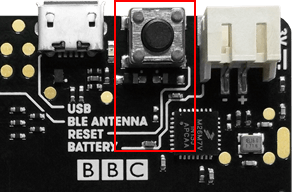
\includegraphics[width=7em,valign=c]{res/mu/060.png}
	
	\end{multicols}

\end{methode}


\begin{remarque}
	Vous devriez avoir un affichage du type\\
		
	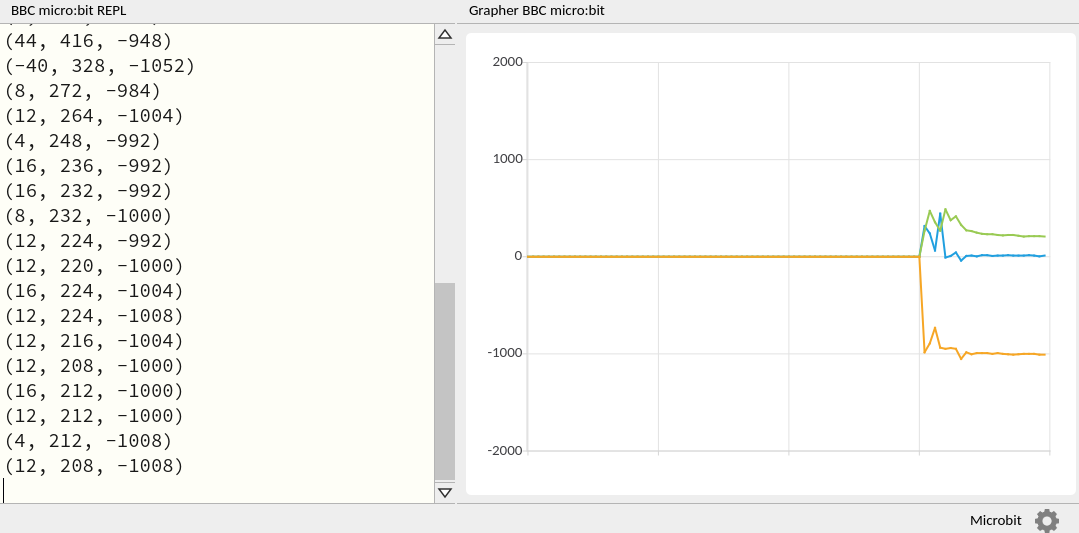
\includegraphics[width=\linewidth,valign=t]{res/mu/090.png}
\end{remarque}
